\chapter{Конструкторский раздел}
\label{cha:design}

В этом разделе будут разработаны алгоритмы моделирования и визуализации галактики типа Sa.

\section{Функциональная модель}

На рисунках \ref{img:idef0_simulation}, \ref{img:idef0_rendering} изображены функциональные модели верхнего уровня для создания модели галактики и её визуализации соответственно.

\begin{figure}[H]
    \centering
    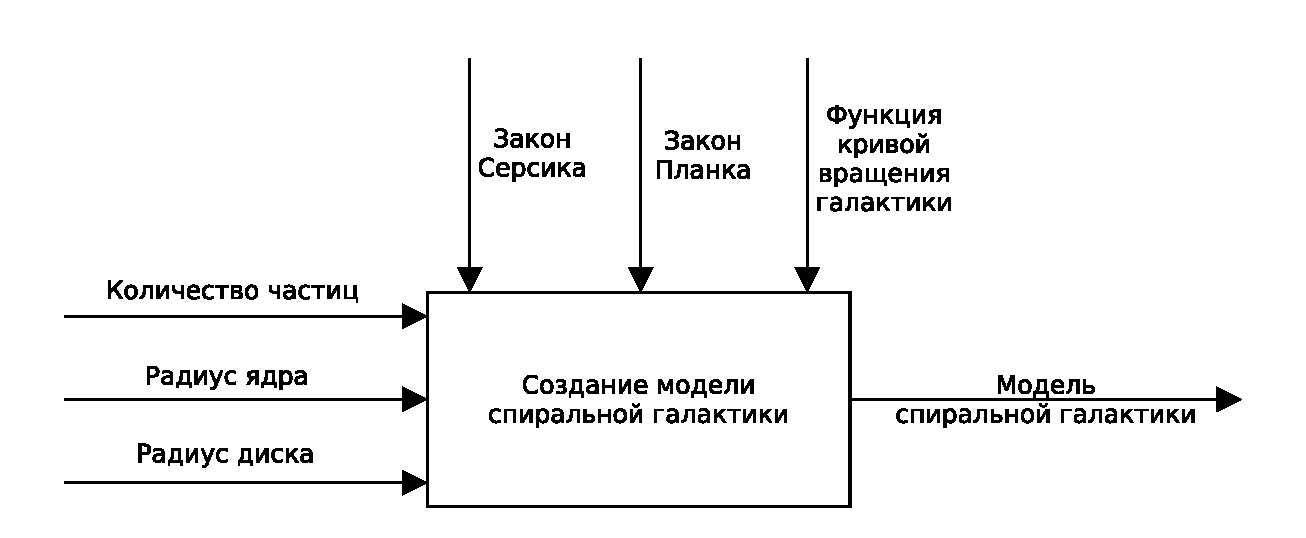
\includegraphics[scale=0.6]{pdf/idef0_simulation.pdf}
    \caption{Функциональная модель IDEF0 верхнего уровня для создания модели галактики}
    \label{img:idef0_simulation}
\end{figure}

\begin{figure}[H]
    \centering
    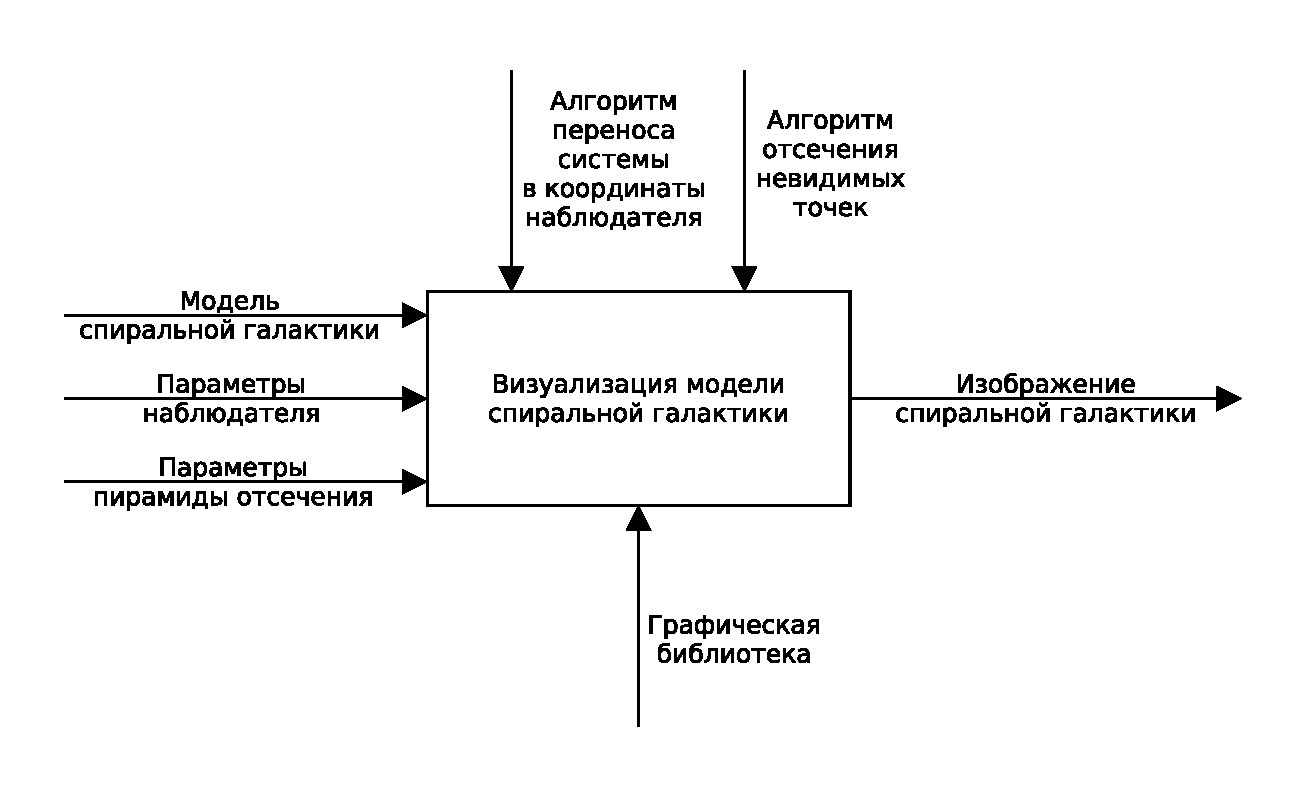
\includegraphics[scale=0.6]{pdf/idef0_rendering.pdf}
    \caption{Функциональная модель IDEF0 верхнего уровня для визуализации модели галактики}
    \label{img:idef0_rendering}
\end{figure}

\section{Описание алгоритмов}

Ниже приведено описание используемых алгоритмов.

\subsection{Вычисление траекторий движения звёзд}

Траекторией звезды является эллипс, который задаётся большой полуосью $a$, эксцентриситетом $e$ и углом поворота вокруг своего центра $\alpha{}$. Тогда малую полуось $b$ можно будет найти по формуле:
\begin{equation}
    b = \sqrt{a^2 \cdot{} (1 - e^2)}
\end{equation}

Ядро спиральной галактики в некоторых аспектах похоже на эллиптическую галактику. Ранее уже говорилось, что к нему применим закон де Вокулёра, но, кроме этого, траектории звёзд внутри ядра приближены к окружностям, как и траектории звёзд внутри эллиптических галактик. Для окружности эксцентриситет равен 0. С увеличением расстояния от центра галактики растёт и эксцентриситет:
\begin{equation}
    e(r) = \left\{ \begin{array}{ll}

    0, & \textrm{$r < 0$} \\
    0 + e_c \cdot{} \frac{r}{R_c}, & \textrm{$r \in [0, R_c]$} \\
    e_c + e_d \cdot{} \frac{r - R_c}{R_d - R_c}, & \textrm{$r > R_d$} \\

           \end{array} \right.
\end{equation}
здесь $e_c$ - эксцентриситет на границе ядра галактики, $e_d$ - эксцентриситет на конце её диска.

Так же необходимо установить зависимость угла поворота $\alpha{}$ от значения полуосей. Так как малая и большая полуось уже связаны, достаточно выбрать только одну из них, например, большую. Пусть $f_{angle}(r)$ - функция угла поворота, зависящая от значения большей полуоси. Скорость роста этой функции влияет на закрученность спиральных ветвей:
\begin{equation}
    f_{angle}(r) = \left\{ \begin{array}{ll}

    0, & \textrm{$r < 0$} \\
    0 + \pi{} \cdot{} \frac{r}{R_c}, & \textrm{$r \in [0, R_c]$} \\
    f_{angle}(R_c) + \pi{} \cdot{} \frac{r - R_c}{R_d - R_c}, & \textrm{$r > R_d$} \\

                   \end{array} \right.
\end{equation}
здесь $R_c$ - радиус ядра спиральной галактики, $R_d$ - радиус диска.

Данные, полученные при измерении процессов, протекающих в природе, характерны своей неточностью. Это означает, что, безусловно, звезды в галактике движутся по траекториям-эллипсам, но очертания этих эллипсов искажены, что следует учитывать при моделировании галактики. Положение звезды на диске задаётся системой параметрических уравнений её траектории:
\begin{equation}
    \left\{ \begin{array}{ll}

        x = a \cdot{} cos(t) \\
        y = b \cdot{} sin(t) \\

    \end{array} \right.
\end{equation}

Чтобы получить немного искажённые значения координат добавим небольшие возмущения:
\begin{equation}
    \left\{ \begin{array}{ll}

        x = a \cdot{} cos(t) + \frac{a}{n} \cdot{} cos(r \cdot{} t) \\
        y = b \cdot{} sin(t) + \frac{b}{n} \cdot{} sin(r \cdot{} t) \\

    \end{array} \right.
\end{equation}
здесь $n$ и $r$ - параметры возмущения. В качестве примера можно взять $n = 40$, $r = 4$. На рисунке \ref{img:densitywaves_analog} приведены траектории движения звёзд с искажёнными траекториями.
\begin{figure}[H]
    \centering
	\includegraphics[scale=0.4]{image/densitywaves_analog.png}
	\caption{Искажённые волны плотности}
	\label{img:densitywaves_analog}
\end{figure}

\subsection{Размещение звёзд в пространстве}
По вертикали звёзды распределяются по нормальному закону. Необходимо определить параметры этого распределения.

Как уже упоминалось, толщина спиральной галактики меньше радиуса её диска в 5-10 раз. Обозначим это число как $k$. Случайной величиной в данном случае является вертикальная составляющая расстояния от звёзды до центра. Следовательно, математическое ожидание такой случайной величины равно 0. По правилу трёх сигм, с вероятностью приблизительно 0.9973 значение нормально распределённой находится в интервале $(m -3\sigma{}, m + 3\sigma{})$. Тогда среднеквадратичное отклонение составляет $\frac{R_d}{3\cdot{}k}$, где $R_d$ - радиус спиральной галактики.

Распределение звёзд по галактическому диску подчиняется закону распределения, функция которого приведена в формуле \ref{eq:F_I}. Для её вычисления потребуется применить метод численного интегрирования. Для ускорения вычисления положения звёзд целесообразно заранее просчитать значения этой функции для набора аргументов от $R_{min}$ до $R_{max}$ с фиксированным шагом, получив таким образом ряд дискретной случайной величины, которую впоследствии можно интерполировать до непрерывной.

\subsection{Создание модели галактики типа Sa}

На рисунке \ref{img:scheme_simulation} приведена схема алгоритма создания модели спиральной галактики.
\begin{figure}[H]
    \centering
    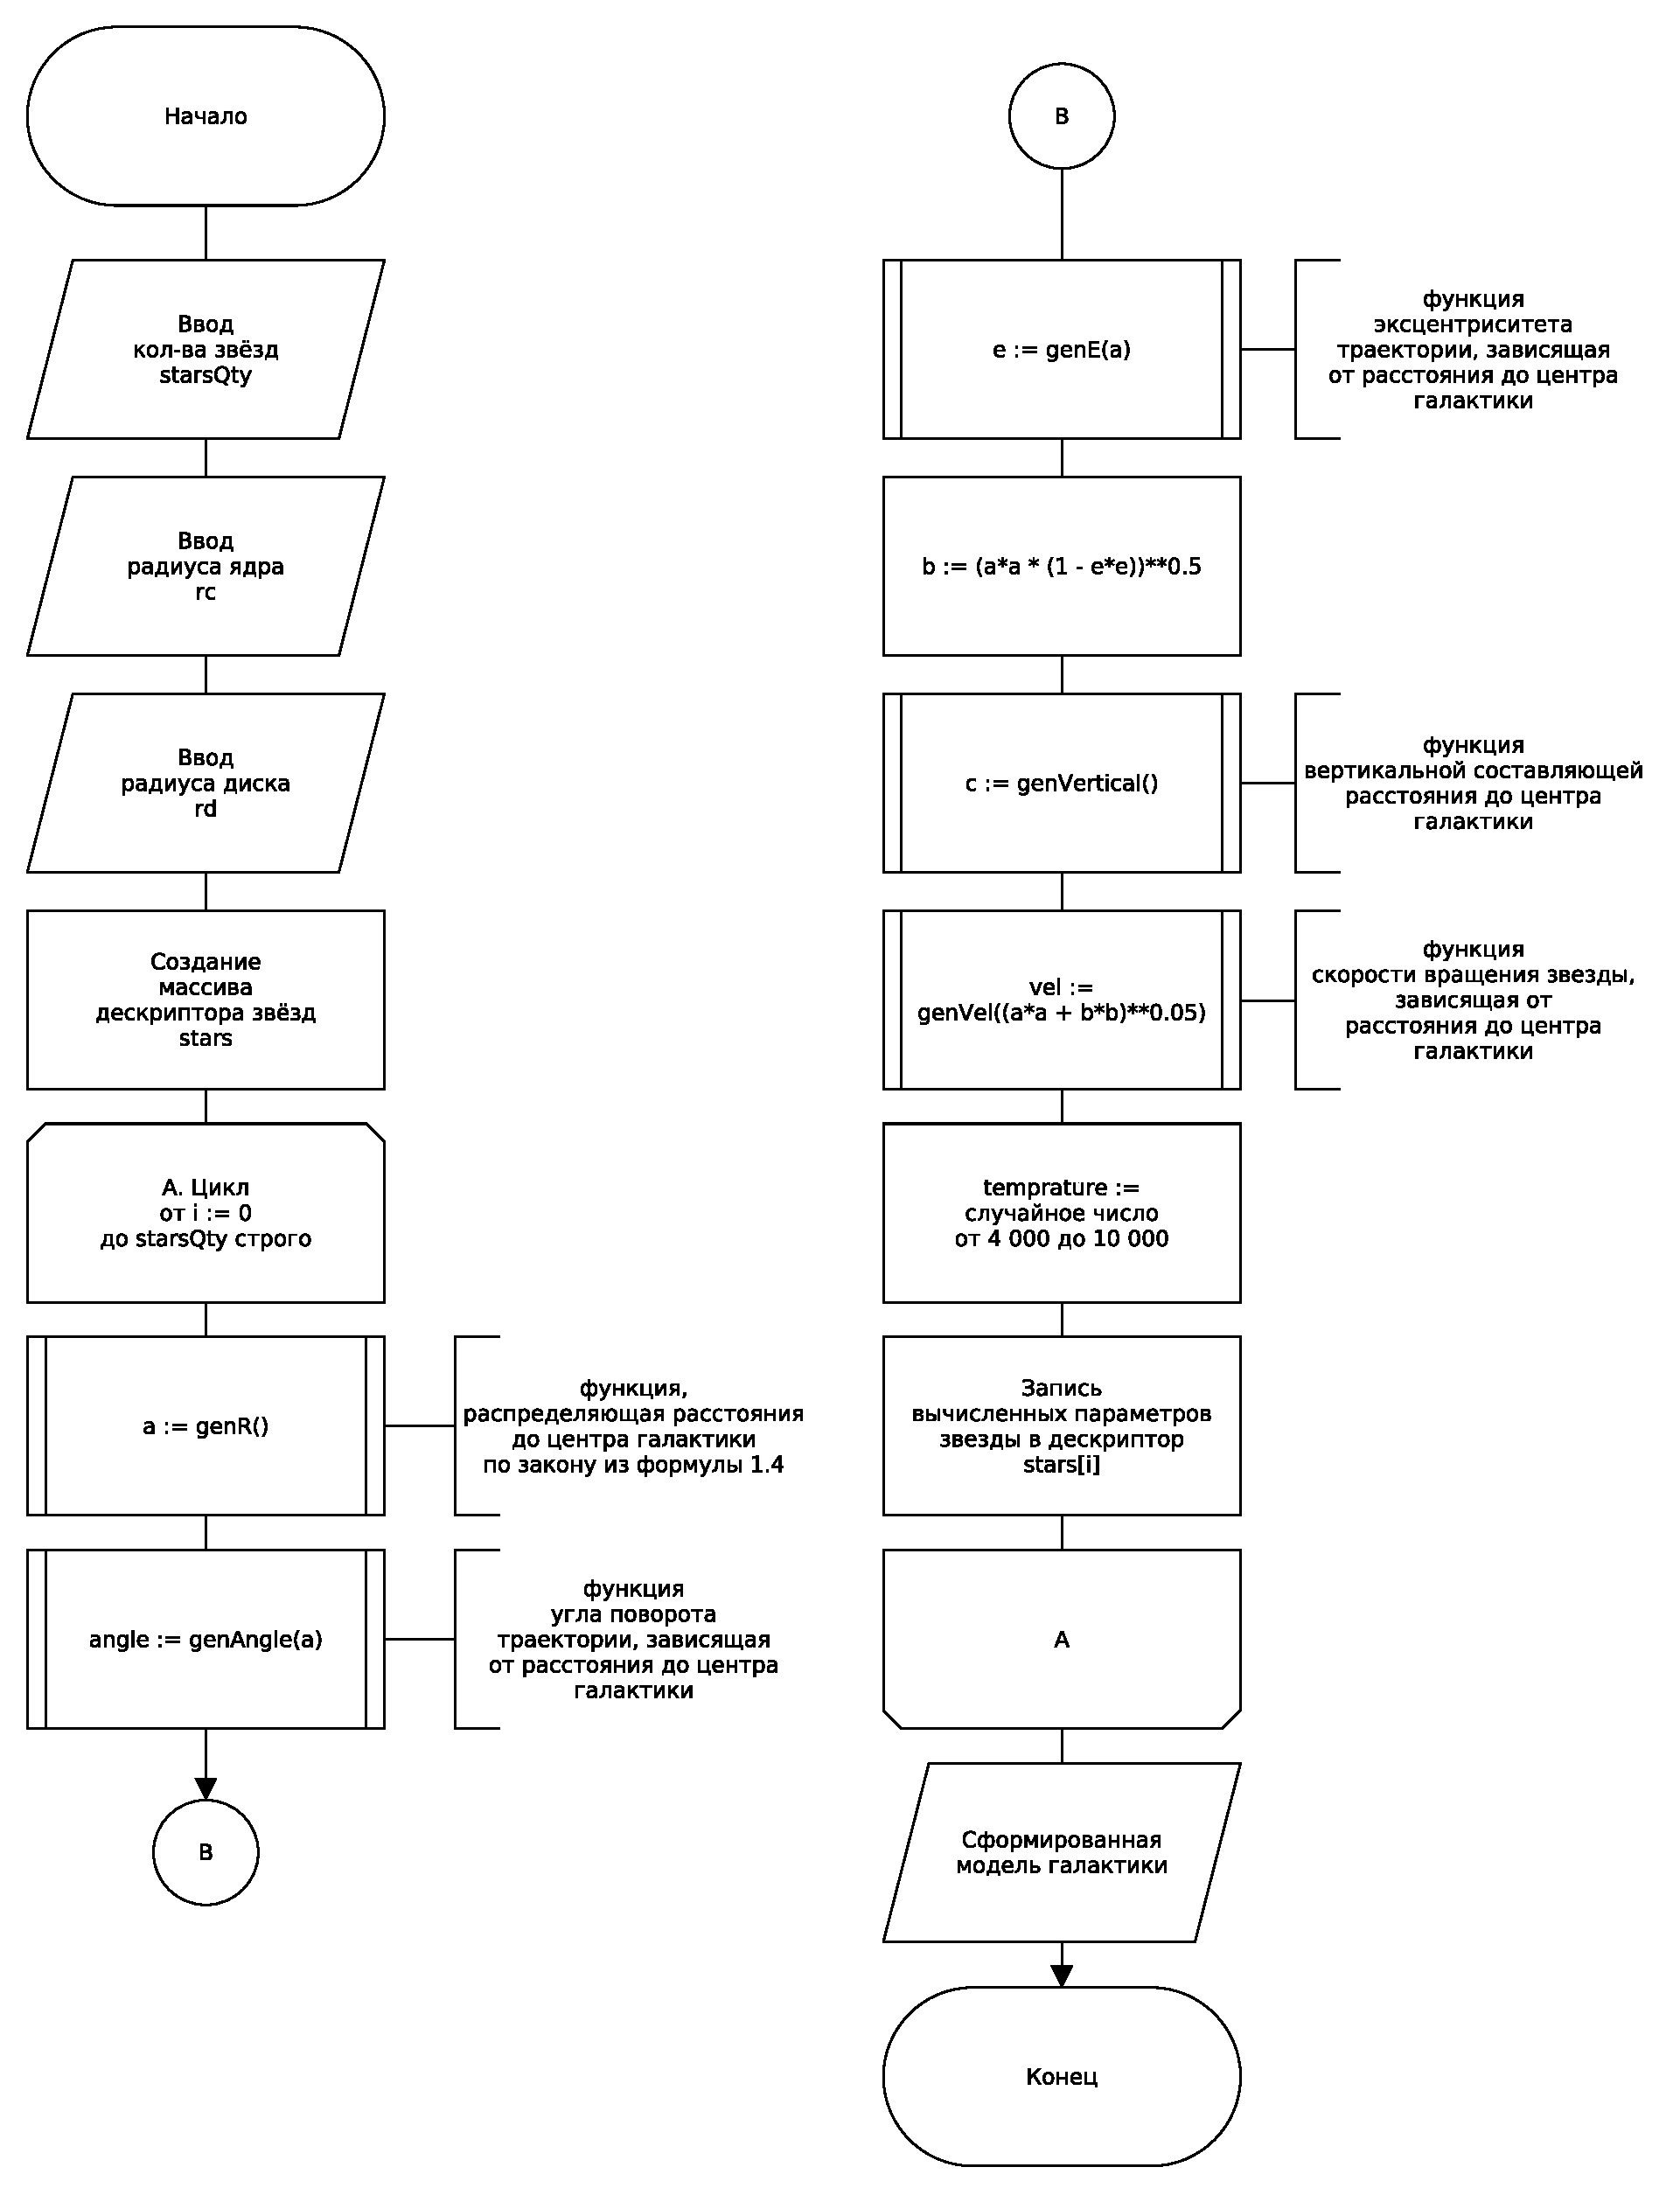
\includegraphics[scale=0.4]{pdf/scheme_simulation.pdf}
    \caption{Схема алгоритма создания модели спиральной галактики}
    \label{img:scheme_simulation}
\end{figure}

\subsection{Визуализация модели галактики типа Sa}

На рисунке \ref{img:scheme_rendering} приведена схема алгоритма визуализации модели спиральной галактики.
\begin{figure}[H]
    \centering
    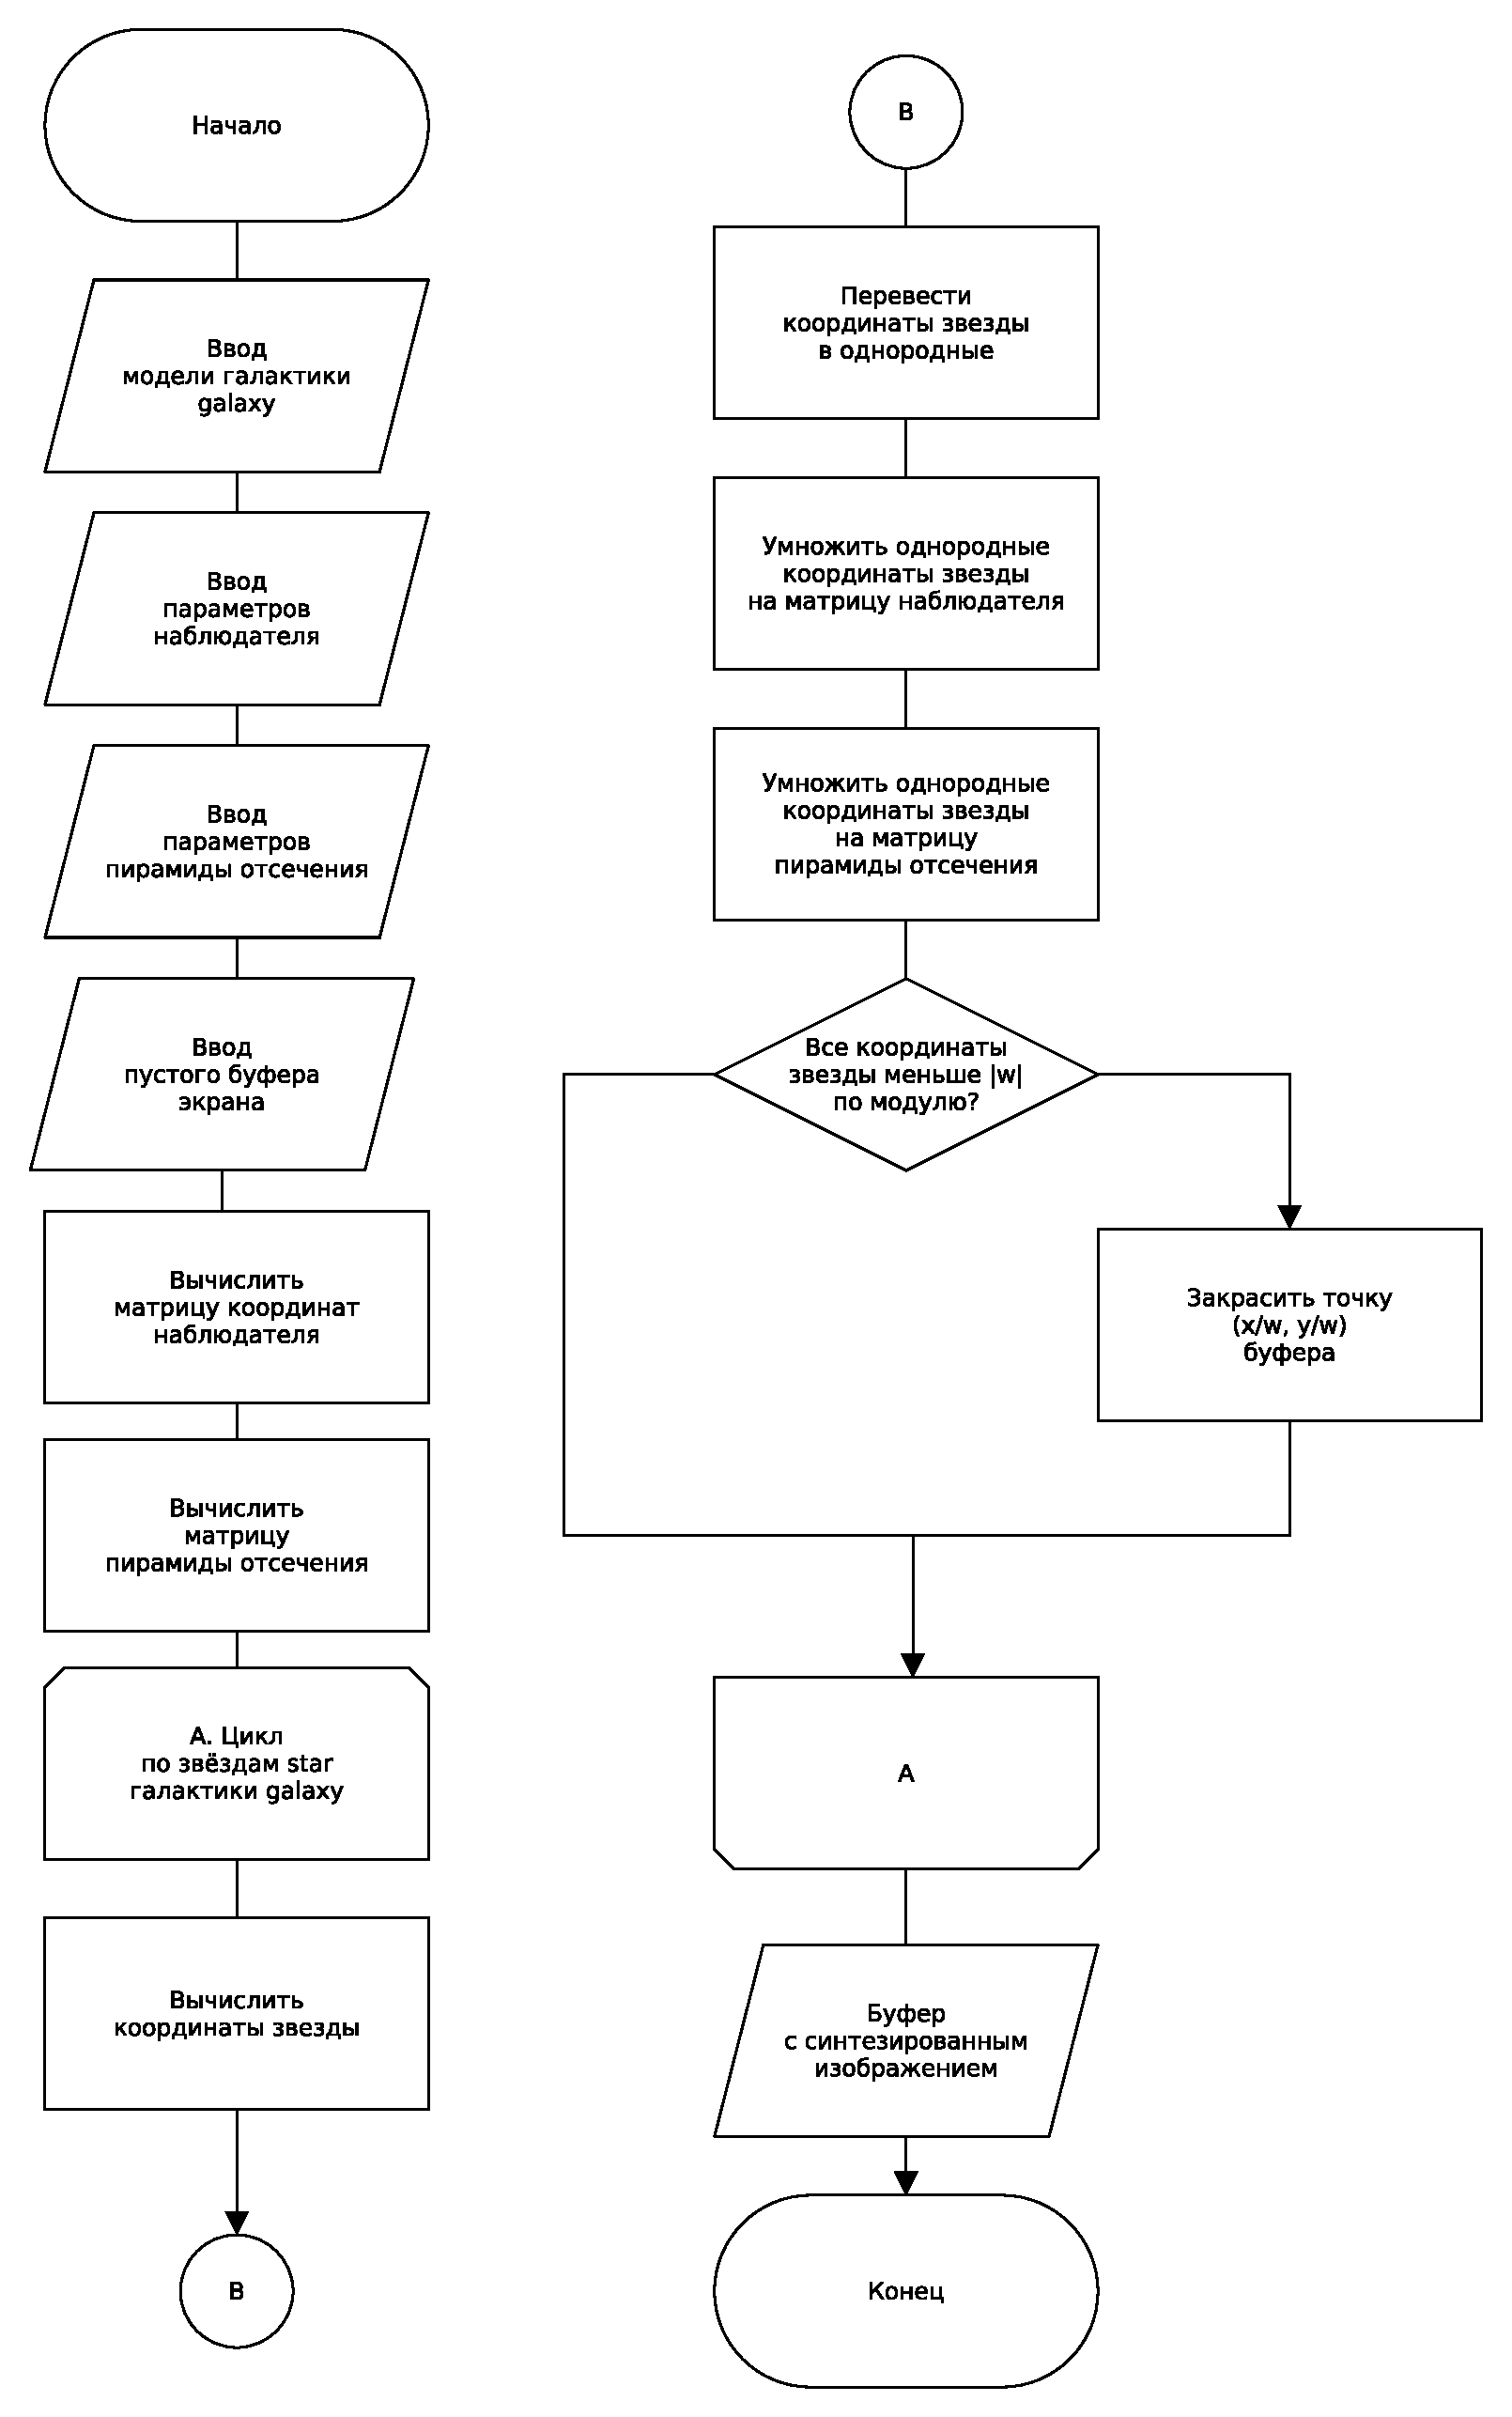
\includegraphics[scale=0.4]{pdf/scheme_rendering.pdf}
    \caption{Схема алгоритма визуализации модели спиральной галактики}
    \label{img:scheme_rendering}
\end{figure}

\section{Выбор используемых типов и структур данных}
Пиксель — это элементарный логический элемент растрового изображения, единица растра. Пиксель характеризуется каким-то определённым цветом, а одна из наиболее удобных и популярных цветовых моделей — RGB, согласно которой цвет определяются тремя целочисленными кодами. Поэтому наиболее удобный тип данных для хранения цвета — сложный тип, объединяющий три целочисленные переменные. В Си-подобных языках программирования такие типы данных называются структурами.

Для хранения информации о изображении нужен некоторый буфер. В качестве буфера удобно использовать обычную матрицу, так как она обладает удобной и быстрой адресацией, а код с её использованием легко читать.

Частицы следует представлять в виде точек, а систему частиц, то есть галактику, в виде структуры, хранящей массив со всеми частицами, количество частиц, радиус звёздного диска, радиус ядра галактики и другие параметры галактики.

\section{Структура программы}
Логически программа разделяется на следующие составляющие:
\begin{itemize}
	\item ядро — реализует базовый, низкоуровневый функционал, который необходим для создания высокоуровневых методов и компонент;
	\item модель — предоставляет доступ к данным и методам, реализует высокоуровненную функциональность;
	\item вид — отправляет данные, полученные от пользователя, и отправляет их пользователю, не взаимодействуя при этом с моделью напрямую;
	\item представитель — отвечает за взаимодействие между пользователем и всей системой, является посредником между моделью и видом.

Данная структура программы призвана обеспечить чёткое разграничение интерфейса и бизнес-логики программы, безопасность потока данных и простоту модифицирования компонент. При этом объектно ориентированный подход является главенствующим при разработки программы.

\end{itemize}

\section{Вывод}
Таким образом, были разработаны алгоритмы создания реалистической модели спиральной галактики и её визуализации, выбраны используемые типы и структуры данных, организована структура программы.

